\documentclass[a4paper, twocolumn]{article}
	\author{Yongqing Liang}
	\title{Improved Surface Carving for Uniform-Texture Video Resizing}
	
\usepackage{amsmath}
\usepackage{amssymb}
\usepackage{enumerate}
\usepackage{graphicx}
\usepackage{float}
\usepackage{color}

\begin{document}
	\maketitle
	
	\section{Overview}
	My work based on [Rubinstein et al. 2008]. And my contributions are below:
	\begin{enumerate}[(1)]
		\item Design an energy function for uniform-texture video.
		\item Optimize structure of graph introduced in [Rubinstein et al. 2008], including discontinued feature and straight-line protection. 
		\item The faster max-flow/min-cut implementation( the fastest is found in [Orlin 2013] ).
		\item Simple but efficient system to video resizing( just an idea).
	\end{enumerate}

	\section{Algorithm}
		\subsection{Energy Map}
			Calculating the energy map of every pixel is two steps. First step is segmentation and track of objects named blocks. Second step is to calculate the energy of each block independently.
			\subsubsection{Segmentation and Track of Object}
			In uniform texture video such as cartoon, there is few feature to describe an object, so, previous algorithms such as deviation filter are useless. Therefore, we introduced a new method to segment object and track it in the video cube.\\
			\linebreak
			Because each object is composed by several color blocks, we will consider blocks instead of object independently. Based on experience, there are two hypothesis. Firstly, the RGB magnitude of each pixel in a specific color block is similar. Secondly, the movement of a color block in two consequence frames is small.\\
			\linebreak
			Supposed a color block is appeared from frame $t_{st}$ to $t_{ed}$. We define $P_i$ as a set of pixels belong to the block in frame $t_i$, where $t_{st} \leqslant t_i \leqslant t_{ed}$ and $$P_i = \{p_1,p_2,p_3,\cdots,p_n\}$$ where $p_j \in P_i$ and $p_j$ contains the spatial information $p_j(x,y)$ of pixel. We use flood-fill algorithm in video cube to segment blocks and track them.\\
			\linebreak
			According to the small movement hypothesis, in most cases, we have $P_i \bigcup P_{i+1} \neq \varnothing $ for a specific color blocks, which means that we could start a seed point in arbitrary pixel inside the block. And it will easily extract complete contour of the block and track the movement of it. We can repeat the flood-fill algorithm for all unvisited pixels to segment the whole video cube.\\
				
			\subsubsection{Saliency of Object}
			We define $m$ as the number of different color blocks in the video cube. We will calculate the energy map of each block in this section. The energy value of pixel is equal to the energy value of block that the pixel is belong to. The higher energy value of block determines the block is more valuable to preserve and vice versa.\\
			\linebreak
			We introduce five arguments to describe the saliency of a color blocks. They are $D_s$(The deviation of numbers of pixels), $D_{cen}$(The deviation of centroid), $D_{cov}$(The deviation of coverage), $D_d$(The deviation of main direction) and $D_f$(The most significant feature of the block). Those five parameters are positive correlation with the energy of block. And we will show the detailed definitions about them bellow.
			
			\paragraph{The deviation of numbers of pixels $D_s$ :}
			When a color block deforms its size during the video cube, the deviation of number of pixels that the block contains in each frame will become large.\\
			\linebreak
			Besides the basic idea, we take some special cases into consider. When the block is not appear from the begin of the video to the end of the video, we set zero as the number of pixels in frame $t_{st}-1$ and $t_{ed}+1$. Decreasing $t_{st}$ and increasing $t_{ed}$ by one at the same time. It means that the block comes from nothing and it finally remains nothing. As the mathematical formula shows below, let $M_s$ as the mean number of pixels about the object from frame $t_{st}$ to frame $t_{ed}$.
			$$M_s = \frac{1}{t_{\Delta}}\sum\limits_{i=t_{st}}^{t_{ed}}\lvert P_i \lvert $$
			$$D_s = \sqrt{\frac{1}{t_{\Delta}-1}\sum\limits_{i=t_{st}}^{t_{ed}}(M_s-\lvert P_i \lvert)^2}$$
			where $t_{\Delta} = t_{ed} - t_{st}$ and $\lvert P_i \lvert$ is the size of the set $P_i$. $P_i$ is a set of pixels which belong to the specific color block in frame $t_i$. Large value of $D_s$ means that the size of block change saliently and it catches more users' attention.
			
			\paragraph{The deviation of centroid $D_{cen}$ :}
			Considering in a specific color block, we define $(c_i(x),c_i(y))$ as centroid of pixels that belong to the block in frame $t_i$.
			$$c_i(x) = \frac{1}{n}\sum\limits_{j=1}^{n}p_j(x)$$
			$$c_i(y) = \frac{1}{n}\sum\limits_{j=1}^{n}p_j(y)$$
			The definition of $p_j$ is shown above and $n=\lvert P_i \lvert$. In this block, we have $\{c_{st},c_{st+1},c_{st+2},\cdots,c_{ed}\}$ that recording the centroid of each frame from $t_{st}$ to $t_{ed}$. Then the deviation of the centroid of the color block is obvious.
			$$M_{cen}(x) = \frac{1}{t_{\Delta}}\sum\limits_{i=t_{st}}^{t_{ed}}c_i(x)$$
			$$M_{cen}(y) = \frac{1}{t_{\Delta}}\sum\limits_{i=t_{st}}^{t_{ed}}c_i(y)$$
			$$D_{cen} = \sqrt{\frac{1}{t_{\Delta}-1}\sum\limits_{i=t_{st}}^{t_{ed}}{\lVert M_{cen}-c_i \lVert}^2}$$
			$\lVert v-u \lVert$ means the Euclidean distance between two coordinates $v$ and $u$.
			Large value of $D_{cen}$ means that the movement of the color block is salient.
			
			\paragraph{The deviation of coverage $D_{cov}$ :}
			We define $cov_i$ as the magnitude of coverage of a specific color block in frame $i$, where $t_{st} \leqslant t_i \leqslant t_{ed}$. As the same consider as the $D_s$ above, we set zero as the coverage value in frame $t_{st}-1$ and $t_{ed}+1$ if it is possible. We can calculate the $cov_i$ as below.
			$$cov_i = \frac{1}{n}\sum\limits_{j=1}^{n}{\lVert p_j-c_i \lVert}^2, \ p_j \in P_i, \ n=\lvert P_i \lvert$$
			$c_i$ is the centroid point of the block in frame $i$. Obviously,
			$$M_{cov} = \frac{1}{t_{\Delta}}\sum\limits_{i=t_{st}}^{t_{ed}}cov_i$$
			$$D_{cov} = \sqrt{\frac{1}{t_{\Delta}-1}\sum\limits_{i=t_{st}}^{t_{ed}}(M_{cov}-cov_i)^2}$$
			The parameter $D_{cov}$ represents another aspect about the size of block compared with $D_{s}$. Taking a ring-like block as an example, the radius of ring turns large along with the video playback. The number of pixels that the block contains may not change, but the coverage of the block vary a lot. So we use $D_{cov}$ to describe this feature.
			
			\paragraph{The deviation of main direction $D_d$ :}
			This parameter is designed to describe the rotation of blocks. When the block rotates rapidly, the value of $D_d$ is large. In each frame, we calculate the direction of each pixel refer to its block centroid and sum them up as the main direction $d_i$ in frame $i$.
			$$d_i = \frac{1}{n}\sum\limits_{j=1}^{n}{f_d(p_j,c_i)}, \ p_j \in P_i, \ n=\lvert P_i \lvert$$
			where the return value of function $f_d(u,v)$ is a vector holds the direction from coordinate $u$ to $v$. $f_d$ is a general representation. Lots of functions such as $atan$ and $atan2$ are available. Similarly,
			$$M_d = \frac{1}{t_{\Delta}}\sum\limits_{i=t_{st}}^{t_{ed}}d_i$$
			$$D_d = \sqrt{\frac{1}{t_{\Delta}-1}\sum\limits_{i=t_{st}}^{t_{ed}}(M_d-d_i)^2}$$
			
			\paragraph{Normalize the parameters ${D'}_*$ :}
			Assume we have $m$ blocks in all. For a specific block $k$, we have four parameters named $D_s^k$, $D_{cen}^k$, $D_{cov}^k$ and $D_d^k$. Before next operators, we need to make a feature scaling normalization on them. Take parameter $D_s$ as an example. We denote $D_d^{max}$ and $D_d^{min}$ as the maximum and the minimum value of all $D_d$.
			$$D_d^{max} = max(D_d^{max}, D_d^k), \ k = 1,\cdots,m$$
			$$D_d^{min} = min(D_d^{min}, D_d^k), \ k = 1,\cdots,m$$
			Then we use the mathematical formula named feature scaling normalization to normalize ${D'}_d$.
			$${{D'}_d}^k = \frac{D_d^k-D_d^{min}}{D_d^{max}-D_d^{min}}, \ k = 1,\cdots,m$$
			The value range of ${D'}_d$ is $[0,1]$.
			
			\paragraph{The most significant feature of block ${D'}_f$ :}
			We have four parameters ${D'}_s$, ${D'}_{cen}$, ${D'}_{cov}$ and ${D'}_d$ to describe features of a specific block so far. The fact is that there are lots of blocks in the video cube. Some of them may rotate, the others may shift in temporal domain. We need to enhance their most significant feature to distinguish the actually salient block from other minor salience blocks. For a specific block, we have
			$${D'}_f = max({D'}_s, {D'}_{cen}, {D'}_{cov}, {D'}_d)$$

			\paragraph{The energy of blocks and pixels $E$}
			The energy function of is a linear combine with those five parameters above.
			$$E = \alpha_1 {D'}_s + \alpha_2 {D'}_{cen} + \alpha_3 {D'}_{cov} + \alpha_4 {D'}_d + \alpha_5 {D'}_f$$
			In our implementation, $\alpha_1 = \alpha_2 = \alpha_3 = \alpha_4 = \alpha_5 = 0.2$ works well. And the value range of $E$ is $[0,1]$.\\
			
		\subsection{Graph Structure}
			We have three subsection in this topic. The first one is based on [Rubinstein et al. 2008] and the others are novel ideas. The basic definition is as the same as mentioned in [Rubinstein et al. 2008]\\
			\linebreak
			We only consider reducing the video size in width. And we construct a grid-like graph $G(V,E)$ from the image in which every node represents a pixel, and connects to its neighboring pixels. $V$ is the set of nodes and $E$ is the set of edges. Each edge in graph has a capacity, also named weight and cost. Sometimes, we call edge as arc. Virtual terminal nodes, $S$(source) and $T$(sink) are created and connected with infinite weight arcs to all pixels of the leftmost and rightmost columns of the image respectively. We define every node in graph except $S$ and $T$ as $v(x,y,t)$, which means the node represent the pixel that is at $x^{th}$ col and $y^{th}$ row in frame $t$.\\
			\linebreak
			An $S/T$ cut $C$ on such a graph is defined as a partitioning of the nodes in the graph into two disjoint subsets $S$ ans $T$ such that $s \in S$ and $t \in T$. The cost of a cut $C = \{S,T\}$ is defined as the sum of the cost of the 'boundary' arcs $(p,q)$ where $p \in S$ and $q \in T$. Note that a cut cost is directed as it sums up the capacity of 'boundary' arcs. That is, arcs in opposite direction do not affect the cost. To define a surface from a cut, we consistently choose the pixels to the left of the cut arcs. The optimal surface is defined by the $minimum \ cut$ which is the cut that has the minimum cost among all valid cuts.\\
			
			\subsubsection{Satisfy Surface Carving}
			There are two rules need to be satisfied.
			
			\paragraph{Represent energy of node:}
			Every node $v(x,y,t)$ has an arc $e$ that connects to its right node $v(x+1,y,t)$. The capacity of arc is the energy value of the node $v(x,y,t)$, which is $E(x,y,t)$. By definition, if the $e$ is in $minimum \ cut$ set, we will deleted the pixel $v(x,y,t)$ in order to reduce the video size in width by one.
			
			\paragraph{The cut passes each row only once:}
			According to graph cut theory, every row has to be cut once in some place in order to generate two subsets. So we build an arc with infinite capacity from node $v(x,y,t)$ to node $v(x-1,y,t)$ if node $v(x-1,y,t)$ exists.\\
			\linebreak
			If a cut pass through one row more than once, some infinite capacity arcs must be included in the cut. This make it an infinite cost cut, which contradicts optimality since it is always possible to cut only horizontal arcs at some column of the grid and achieve a finite cost cute.\\
			
			\subsubsection{Feature of discontinued surface}
			The graph structure proposed by [Rubinstein et al. 2008] has diagonal arcs to guarantee the resulting cut will be a continuous function over relevant domain. In our experiments, we found that when the object moving quickly more than one pixel per frame, the hypothesis that pixels of seams must be connected which proposed in [Rubinstein et al. 2008] is not applicable. In our work, we add penalty arcs to preserve spatial and temporal coherence instead of old diagonal arcs.
			
			\subsubsection{Straight-line protection}
			By definition, we have that all nodes to the left of the cut labeled $S$ and all nodes to the right of the cut labeled $T$. And the cost of a cut will only consider arcs directed from nodes labeled $S$ to nodes labeled $T$. Hence, considering in spatial plane, we assign a upward vertical arc between $v(x,y,t)$ and $v(x,y-1,t)$ as a spatial penalty arc. We also assign a downward vertical arc between $v(x,y,t)$ and $v(x,y+1,t)$ as a spatial penalty arc too. The graph structure in temporal plane is similar and there are a backward and a forward penalty arcs.\\
			\linebreak
			We define an upward penalty capacity $c$ of arc $v(x,y,t) \rightarrow v(x,y-1,t)$ as follows.
			$$c = \lvert \frac{\partial}{\partial x}I_t(x,y)\lvert$$
			where $I_t$ is the $i^th$ frame in the video. If there is a sharp change in the side of pixel $v(x,y,t)$, the penalty capacity $c$ will be large. And it will prevent the cut from passing through it.\\
			\linebreak
			Figure 1 shows more details. If the cut tries to delete two pixels $v(5,1,t)$ and $v(1,2,t)$, it will sum up 3 cost of penalty arcs, which are three dashed blue line. If there is a sharp change between $v(5,1,t)$ and $v(1,2,t)$, the cost of penalty arcs will be large. And it will prevent the bad curve happening efficiently.\\
			\linebreak
			Figure 2 is a bad curve example in horizontal dimension from [Rubinstein et al. 2008]. The other penalty arcs are built as the same as the upward arc defined above.
			\begin{figure}
				\begin{center}
				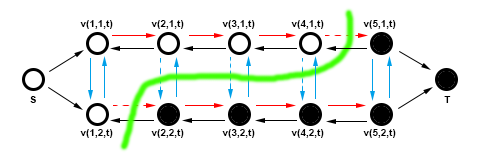
\includegraphics[width=\linewidth]{Figure1.png}
				\caption{The green curve is a cut. All white nodes label $S$ and all black nodes label $T$. Black arcs are infinite weights. Blue arcs are penalty arcs. The arcs with dashed line are 'boundary' arcs. And they will be summed up as the cost of the curve.}
				\end{center}
			\end{figure}
			\begin{figure}
				\begin{center}
				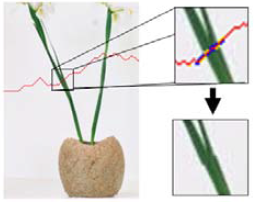
\includegraphics[width=\linewidth]{Figure2.png}
				\caption{A bad curve example in horizontal dimension from [Rubinstein et al. 2008]. Our work can prevent this bad curve.}
				\end{center}
			\end{figure}
		
		\subsection{Speed Up Graph Cuts}
		This method has been mentioned in [Rubinstein et al. 2008] and it works well.\\
		\linebreak
		To improved efficiency, we employ a banded multi-resolution method, similar to the one described in [Lombaert et al. 2005]. An approximate minimal cut is first computed on the coarsest graph, and then iteratively refined at higher resolutions. Coarsening is performed by sampling the graph both spatially and temporally, while refinement is done by computing graph cut on a narrow band induced by the cut that was computed at the coarser level. Figure 3 shows more details.
		\begin{figure}
			\begin{center}
			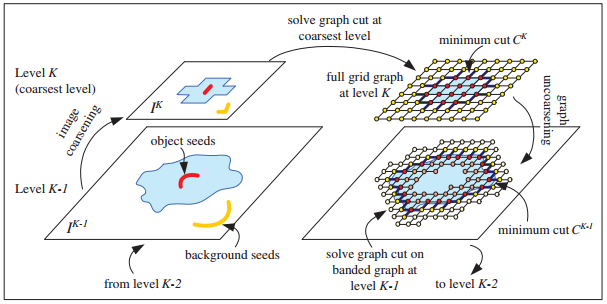
\includegraphics[width=\linewidth]{Figure3.png}
			\caption{Multilevel banded graph cut algorithm from [Lombaert et al. 2005].}
			\end{center}
		\end{figure}
	
	\section{Implementation}
		
		This part of code isn't implemented in the code due to time limited. Just some ideas.
		
		\subsection{Combine Scaling and Seams}
		There is a wide discussion about relationship between seam carving, scaling and cropping. I am trying to take full advantage of scaling and seam carving approaches to address the problem of fitting content to display well.\\
		\linebreak
		If we want to reduce the video size from 100$\times$100\textit{px} to 100$\times$50\textit{px}. Perhaps the unimportant ingredients of the video is less than half. Traditional surface curving may distort the content of video. Here is a novel method works well.\\
		\linebreak
		We can uniformly rescale the video size to 75$\times$75\textit{px}. Then we enlarge the video size in horizontal dimension to 100$\times$75\textit{px} by Seam Carving. Finally, we reduce the video size in vertical dimension to the preset size 100$\times$50\textit{px}.
		
		\subsection{Compress Similar Frames}
		In high resolution video, the $fps$ value usually more than 30. In our experiment, we find that the difference between two consecutive frames is trivial in most cases. So we can take one frame as a representation of similar frames and set the energy value of the region with changes with a average energy value among those frames. This method can reduce the nodes in graph and make computation of graph cuts more efficient.
		
		\subsection{User Interaction}
		Because of the good segmentation, user interaction can mark the important/unimportant area in a few key frames(usually two or three) in energy map. And it will make a better result video.
		
		\subsection{Process Framework}
		\begin{enumerate}[(1)]
			\item Input the origin video and preset size. Supposed reduce width.
			\item Compress the similar frames. (Sec. 3.2)
			\item Uniformly rescale the video size. (Sec. 3.1)
			\item Segment and track the object. (Sec 2.1.1)
			\item Calculate the energy map. (Sec. 2.1.2)
			\item User interaction refine the energy map. (Sec. 3.3)
			\item Reduce the width.
				
				\subitem Build video pyramid. (Sec. 2.3)
				\subitem Build graph with energy map and penalty arcs. (Sec. 2.2)
				\subitem Graph cut in coarse level and refine it at higher resolutions level. (Sec. 2.3)
				\subitem Delete the pixels from graph cut.
			\item Enlarge the height.
				\subitem Similar to 'Reduce the width' but the final step is duplicating the pixels from graph cut.
			\item Restore frames because of Step (2).
			\item Algorithm finished.
			
		\end{enumerate}
	
	\section{Related Work}
	
		\subsection{[Rubinstein et al. 2008]}
		\begin{enumerate}[(1)]
			\item The cut of this algorithm is strict spatial and temporal connected. My cut is discontinuous and my graph has penalty arcs.
			\item It take 10 to 20 minutes for 400$\times$300\textit{px}, 400 frames reducing 50\textit{px}. My algorithm needs less than 10 minutes.
			\item The algorithm is designed for un-uniform texture video resizing. My energy function is designed for uniform texture video.
			\item Both algorithms are global optimization.
		\end{enumerate}
		
		\subsection{[Lombaert et al. 2005]}
		\begin{enumerate}[(1)]
			\item Adopting multilevel banded graph cut.
		\end{enumerate}
		
		\subsection{[Grundmann et al. 2010]}
		\begin{enumerate}[(1)]
			\item Adopting discontinuous cut idea.
		\end{enumerate}

		\subsection{[Yan et al. 2013]}
		\begin{enumerate}[(1)]
			\item Adopting penalty ideas.
			\item It is local optimal algorithm. My work is global optimization.
		\end{enumerate}
		
		\subsection{[Hu et al. 2010]}
		\begin{enumerate}[(1)]
			\item Similar to [Yan et al. 2013] but combine local and global optimization. Just so-so.
			\item Inspire my frame compression.
		\end{enumerate}
		
		\subsection{[Krähenbühl et al. 2009]}
		\begin{enumerate}[(1)]
			\item There are two main methods for video resizing. One is based on seam carving, the other is based on image warp. This is a typical implementation based on image warp.
			\item It is a frame by frame local optimization. Mine is a global optimization.
			\item It is a real-time algorithm. Better than mine.
		\end{enumerate}
	
	\section{Future Work}
	\begin{enumerate}[(1)]
		\item Write down my ideas into code after discussion.
		\item Reading further work by Michael Rubinstein. Two papers named \textit{Multi-operator Media Retargeting} and \textit{Riesz pyramids for fast phase-based video magnification}. The website is {http://www.faculty.idc.ac.il/arik/SCWeb/multiop/index.html}
		\item Discuss next research stage with Professor Jin.
		\item Reading more efficient algorithm of max-flow problem if necessary.
	\end{enumerate}
	
	\section{Reference}
		\begin{enumerate}[(1)]
			\item Rubinstein M, Shamir A, Avidan S. Improved seam carving for video retargeting[C]//ACM transactions on graphics (TOG). ACM, 2008, 27(3): 16.
			
			\item Lombaert H, Sun Y, Grady L, et al. A multilevel banded graph cuts method for fast image segmentation[C]//Computer Vision, 2005. ICCV 2005. Tenth IEEE International Conference on. IEEE, 2005, 1: 259-265.
			
			\item Grundmann M, Kwatra V, Han M, et al. Discontinuous seam-carving for video retargeting[C]//Computer Vision and Pattern Recognition (CVPR), 2010 IEEE Conference on. IEEE, 2010: 569-576.
			
			\item Yan B, Sun K, Liu L. Matching-area-based seam carving for video retargeting[J]. Circuits and Systems for Video Technology, IEEE Transactions on, 2013, 23(2): 302-310.
			
			\item Krähenbühl P, Lang M, Hornung A, et al. A system for retargeting of streaming video[J]. ACM Transactions on Graphics (TOG), 2009, 28(5): 126.
			
			\item Hu Y, Rajan D. Hybrid shift map for video retargeting[C]//Computer Vision and Pattern Recognition (CVPR), 2010 IEEE Conference on. IEEE, 2010: 577-584.
		\end{enumerate}
			
			
\end{document}